% !TEX encoding = UTF-8 Unicode
\documentclass[12pt]{article}
\usepackage[T2A]{fontenc}
\usepackage[utf8]{inputenc}
\usepackage[english, russian]{babel}

\usepackage{graphicx}
\graphicspath{{images/}}
\usepackage{amsmath, amsthm, amssymb, thmtools}
\usepackage{algorithm}
\usepackage{algpseudocode}
\usepackage{cite}

\usepackage{geometry}
\usepackage{indentfirst}
\textheight = 24cm
\textwidth = 16cm
\oddsidemargin = 0cm
\topmargin = -1.5cm
\parindent = 24pt
\parskip = 0pt
\flushbottom
\linespread{1.3}

\declaretheorem[style = definition, numbered = no, name = Определение]{definition}
\declaretheorem[style = plain, name = Лемма]{lemma}
\declaretheorem[style = plain, name = Теорема]{theorem}

\begin{document}
\begin{titlepage}
\begin{center}

	\includegraphics[width=50mm]{msu.eps}
	
	\bigskip

	Московский государственный университет имени~М.~В.~Ломоносова\\
	Факультет Вычислительной Математики и Кибернетики\\
	Кафедра Математических Методов Прогнозирования\\[30mm]

	\textsf{\large
      ВЫПУСКНАЯ КВАЛИФИКАЦИОННАЯ РАБОТА\\[10mm]
      \textbf{
        Слияние перекрывающихся триангуляций Делоне на основе минимальных остовных деревьев
      }
    }\\[30mm]
	
	\begin{flushright}
      \parbox{0.5\textwidth}{
        \raggedleft
        \textbf{Выполнила:}\\
        студентка 417 группы\\
        Готман Мария Леонидовна\\[5mm]
        \textbf{Научный руководитель:}\\
        д.т.н., профессор\\
        Местецкий Леонид Моисеевич
      }
    \end{flushright}	
	
	\vspace{\fill}
	Москва, 2015
\end{center}
\end{titlepage}

\newpage

\tableofcontents

\newpage
\begin{abstract}
В данной работе рассмотрен алгоритм слияния двух триангуляций Делоне,
причем множества, на которых заданы исходные триангуляции, допускают полное перемешивание.
Алгоритм, решающий данную задачу, имеет линейную сложность в худшем случае.
Метод основан на построении минимальных остовных деревьев исходных триангуляций
при помощи алгоритма Черитона-Тарьяна.
Это является ключевой частью алгоритма, за счет чего достигается его линейная сложность.
\end{abstract}

\newpage
\section{Введение}
Рассматривается задача слияния двух триангуляций Делоне, линейная разделимость исходных облаков точек которых не предполагается.
Впервые задача построения триангуляции Делоне была рассмотрена в 1934 году российским математиком Борисом Делоне.
На практике триангуляции Делоне применяются во многих прикладных задачах:
сравнение 3D поверхностей, интерполяция разреженных геонаучных данных,
аппроксимация географических поверхностей на плоскости и т.д.

Несмотря на то, что построение триангуляции Делоне является распространенной задачей в вычислительной геометрии \cite{Skvortsov},
слияние неразделенных триангуляций исследовано мало.
Такую задачу решают обычно одним из следующих способов.
Первый способ основан на том, что информация об исходных триангуляциях никак не учитывается и искомая триангуляция строится
по объединенному множеству точек с нуля. Сложность такого алгоритма $O(n\log n)$ в худшем случае.
Такая асимптотика достигается при помощи парадигмы <<разделяй и властвуй>>.
Множество точек разделяется пополам, ещё раз пополам и так далее, пока в подмножестве не останутся 2 или 3 точки,
на которых строится тривиальная триангуляция в виде линии или треугольника.
Затем происходит процесс слияния разделенных триангуляций за линейное время.
Второй способ разрушает только одну триангуляцию,
затем последовательно добавляет по одной точке разрушенной триангуляции с помощью инкрементного алгоритма.
Такой подход имеет сложность $O(n^2)$ в худшем случае.

Как видно, оба подхода не используют всю информацию о исходных триангуляциях,
поэтому естественно кажется, что существует алгоритм, помогающий осуществить слияние за линейное время.
Основанием для этого служит существование алгоритма Ли-Шехтера \cite{Lee},
который производит слияние для линейно разделимых триангуляций за время $O(n)$.
Также существует алгоритм Киркпатрика, которые сливает две диаграммы Вороного за линейное время.
Использование этого алгоритма также не является эффективным решением данной задачи.
Получается много временных затрат на переход к диаграммам Вороного и обратно.

В данной работе рассматривается линейный алгоритм слияния триангуляций Делоне.
Алгоритм основан на построении минимальных остовных деревьев (МОД) исходных триангуляций.
Известно, что МОД является подграфом триангуляции Делоне.
Эта информация используется при поиске новых ребер, соединяющих две исходные триангуляции.
Если найдено ребро, соединяющее точки из разных исходных триангуляций, называемое стартером,
то можно строить <<швы>>, соединяющие исходные триангуляции,
и <<разрезы>>, содержащие ребра, которые перестали удовлетворять условию Делоне.
Подзадача построения швов и разрезов является наиболее сложно осуществимой с технической точки зрения.
Поиск стартеров технически проще, но понимание его математического обоснования
требует должных усилий.

\section{Терминология и постановка задачи}

\subsection{Основные определения}
Пусть на евклидовой плоскости задано $\textbf{S}$ --- множество из не менее трех точек, не все из которых лежат на одной прямой.
Используя \cite[стр.~7-8]{Skvortsov}, \cite{MestOverlap}, введем ряд ключевых определений которые понадобятся нам для дальнейшего понимания задачи.

Точки, входящие во множество $\textbf{S}$, будем называть {\itshape сайтами}.
{\itshape Триангуляцией} конечного множества точек $\textbf{S}$ называется планарный граф с вершинами из $\textbf{S}$,
все внутренние области которого являются треугольниками.
Триангуляция называется {\itshape выпуклой}, если минимальный многоугольник, охватывающий все ее треугольники, будет выпуклым.
Далее под термином {\itshape грань} будем понимать только конечную треугольную грань триангуляции.
Ребро и грань называются {\itshape инцидентными}, если они имеют две общие вершины.
Ребра, инцидентные одной грани, называются {\itshape смежными}.
Ребро, имеющее менее двух инцидентных граней, называется {\itshape открытым}.

Окружность называется {\itshape пустой}, если она не содержит внутри себя сайтов.
Прямая линия, по одну сторону от которой нет сайтов, называется {\itshape несобственной} пустой окружностью.
Окружность, проходящая через сайт, называется {\itshape инцидентной} этому сайту.
{\itshape Ребром Делоне} называется ребро, инцидентные сайты которого имеют общую пустую инцидентную окружность.
{\itshape Гранью Делоне} называют грань, вершины которой имеют общую пустую инцидентную окружность.

Дадим два эквивалентных определения:

\begin{definition}
{\itshape Триангуляцией Делоне (ТД) $Del(\textbf{S})$} множества точек $\textbf{S}$ называется выпуклая триангуляция,
у которой описанная окружность каждой треугольной грани является пустой,
т.е. все грани которой являются гранями Делоне.
\end{definition}

\begin{definition}
{\itshape Триангуляцией Делоне} множества точек $\textbf{S}$ называется выпуклая триангуляция,
у которой для каждого ребра существует пустая инцидентная сайтам-вершинам окружность,
т.е. все ребра которой являются ребрами Делоне.
\end{definition}

{\itshape Пучком} сайта $p \in \textbf{S}$ называют множество ребер триангуляции, инцидентных сайту $p$.
Пучок сайтов будем представлять в виде двунаправленного циклического списка сайтов $p_1, \ldots, p_k$,
смежных с $p$ в триангуляции, так чтобы они шли в направлении обхода против часовой стрелки относительно $p$.

\subsection{Постановка задачи}
Задача слияния двух перекрывающихся триангуляций Делоне ставится следующим образом.
Даны два конечных линейно неразделимых множества сайтов $\textbf{B}$ и $\textbf{W}$ (допускается их полное перемешивание),
а также их триангуляции Делоне $Del(\textbf{B})$ и $Del(\textbf{W})$.
Нужно построить триангуляцию Делоне на объединенном множестве сайтов $Del(\textbf{B} \cup \textbf{W})$.

Будем считать, что сайты раскрашены в два цвета: множество черных сайтов $\textbf{B}$ и множество белых сайтов $\textbf{W}$.
Триангуляции множеств $\textbf{B}$ и $\textbf{W}$ будем называть исходными,
искомую триангуляцию $Del(\textbf{B} \cup \textbf{W})$ будем называть объединенной.
Пример исходных данных и искомой триангуляции приведен на рис. \ref{pic:model_data}.

\begin{figure}[htb!]
	\begin{minipage}[h]{0.49\linewidth}
		\center{\includegraphics[width=1\linewidth]{model_data.png}}
	\end{minipage}
	\hfill
	\begin{minipage}[h]{0.49\linewidth}
		\center{\includegraphics[width=1\linewidth]{model_res.png}}
	\end{minipage}
	\caption{Исходные триангуляции и объединенная триангуляция}
	\label{pic:model_data}
\end{figure}

Нижняя оценка для задачи построения триангуляции Делоне множества точек $\textbf{S}$ известна
и имеет сложность $O(n\log n)$, где $n = |\textbf{S}|$ \cite[лекции 10-11]{Lectures}.
Такую сложность имеет, например, алгоритм, основанный на парадигме <<разделяй и властвуй>> \cite[стр.44-45]{Skvortsov}, \cite{Lee}.
Этот алгоритм имеет сложность $O(n\log n)$ в среднем и худшем случае.
Такой алгоритм позволяет производить слияние разделенных триангуляций Делоне за линейное по числу точек время.
Однако вопрос о слиянии перекрывающихся триангуляций Делоне остается открытым.
Возможным подходом является построение объединенной триангуляции на множестве $\textbf{B} \cup \textbf{W}$
без учета информации о исходных триангуляциях.
Такой подход не является эффективным.
В \cite{MestOverlap} доказана теоретическая оценка времени слияния неразделенных триангуляций Делоне, равная в худшем случае $O(n)$.
В работе \cite{Dyshkant} был реализован линейный алгоритм построения минимальных остовных деревьев,
которые используются при построении объединенной триангуляции, 
но алгоритм слияния триангуляций в среднем имел асимптотику $O(n)$, в худшем случае $O(n\log n)$.
В настоящей работе будет описан линейный алгоритм слияния триангуляций Делоне,
проведены эксперименты, доказывающие его теоретическую оценку.

\section{Описание алгоритма}
В данном разделе введем основные понятия, связанные с разрушением ребер в исходных триангуляциях
и построением новых ребер объединенной триангуляции,
а также дадим общую схему алгоритма слияния перекрывающихся триангуляций Делоне \cite{MestOverlap}.

В объединенной триангуляции Делоне $Del(\textbf{B} \cup \textbf{W})$ существуют ребра двух типов:
одноцветные, которые были взяты из исходных триангуляций, и разноцветные, сайты-вершины которых взяты из разных исходных триангуляций.

Множество вершин и ребер (ребер и граней) называется {\itshape связным}, если для любой пары элементов этого множества
существует цепь из попарно инцидентных вершин и ребер (ребер и граней), принадлежащих этому множеству.

В объединенной триангуляции существуют максимальные связные одноцветные подмножества вершин и ребер,
переходящие без изменений из исходных триангуляций, которые будем называть {\itshape лоскутами}.
Ребра и грани, не вошедшие в лоскуты, должны быть разрушены.
Такие связные подмножества будем называть {\itshape разрезами}.
При построении разрезов будут удалены некоторые грани, что приведет к образованию открытых ребер.
Связную цепочку вершин и открытых ребер, состоящих из ребер одного цвета, будем называть {\itshape краем}.
Максимальные связные подмножества разноцветных ребер и граней объединенной триангуляции будем называть {\itshape швами}.
Разноцветные ребра будем называть {\itshape стежками}.

При данных определениях построение объединенной триангуляции Делоне состоит из нескольких частей: построения разрезов,
выделения лоскутов исходных триангуляций и построения швов.
Каждый шов соединяет два разноцветных края, образованных после разрушения ребер, вошедших в разрезы.
В начале работы алгоритма краями исходных триангуляций являются их выпуклые оболочки.
По мере построения разрезов и швов количество краев меняется
(увеличивается при построении разрезов и уменьшается при построении швов).
В объединенной триангуляции остается только один край --- граница выпуклой оболочки.

{\itshape Стартером} будем называть пару разноцветных сайтов, образующих ребро Делоне,
еще не включенное в объединенную триангуляцию.
Стартер нужен для запуска процесса построения разреза и шва.
Построение смежных стежков для стартера можно вести по разные стороны от него.
Для определенности будем полагать, что стартер имеет левый и правый сайты,
построение стежка происходит в направлении перед стартером.
На рис. \ref{pic:dir} черная жирная линия обозначает стартер, жирная пунктирная новый стежок, построенный в направлении перед стартером.

\begin{figure}[htb!]
	\begin{minipage}[h]{0.49\linewidth}
		\center{\includegraphics[width=1\linewidth]{starter.png}}
	\end{minipage}
	\hfill
	\begin{minipage}[h]{0.49\linewidth}
		\center{\includegraphics[width=1\linewidth]{direct_starter.png}}
	\end{minipage}
	\caption{Построение новых стежков}
	\label{pic:dir}
\end{figure}

Шов может быть двух типов.
{\itshape Разомкнутым} швом называется шов, имеющий два стежка, принадлежащих выпуклой оболочке объединенной триангуляции,
то есть принадлежащих граничным ребрам $Del(\textbf{B} \cup \textbf{W})$.
{\itshape Циклическим} называется шов, имеющий только внутренние ребра объединенной триангуляции.

В процессе построения разомкнутого шва сначала находим одну его часть,
затем продолжаем движение по другую сторону стартера и находим оставшуюся часть разреза.
В циклическом шве в некоторый момент времени стартер совпадет с новым стежком,
на этом построение шва будет закончено.

Введем понятие минимального остовного дерева.
{\itshape Минимальным остовным деревом (МОД)} триангуляции Делоне называется ее связный подграф,
имеющий наименьшую суммарную длину ребер.
Пусть на плоскости задано $N$ точек.
{\itshape Евклидовым МОД (ЕМОД)} называется связный подграф,
вершинами которого являются все $N$ точек, суммарная длина всех ребер которого минимальна.
Известно, что МОД ТД является евклидовым минимальным остовным деревом для множества сайтов ТД \cite[стр. 229, 277]{Preparata}.
МОД исходных триангуляций Делоне понадобятся в процессе построения стартеров.

\subsection{Общая схема алгоритма}
\begin{enumerate}
	\item Построить минимальные остовные деревья для обеих исходных триангуляций.
	\item Построить начальный стартер
	\item \label{alg1:l1} Построить разрез и шов
	\begin{enumerate}
		\item Объявить стартер текущим стежком
		\item Провести коррекцию одноцветных ребер (построение разреза)
		\item \label{alg1:l2} Построить новый стежок
		\item Если построить новый стежок не удалось, развернуть стартер и перейти к пункту \ref{alg1:l1}
		\item Если построить новый стежок не удалось во второй раз, закончить построение шва
		\item Удалить ребра, пересекающие новую грань
		\item Проверить совпадение со стартером, в случае совпадения закончить построение шва, иначе перейти к шагу \ref{alg1:l2}
	\end{enumerate}
	\item Поиск очередного стартера
	\item Если стартер найден, перейти к пункту \ref{alg1:l1}, иначе закончить работу алгоритма
\end{enumerate}

\subsection{Выбор структуры данных}
Выбор структуры данных сильно влияет на сложность дальнейших вычислений.
В книге \cite[стр. 11-17]{Skvortsov} описаны несколько структур данных, которые могут быть использованы для решения данной задачи.

\begin{figure}[htb!]
	\center{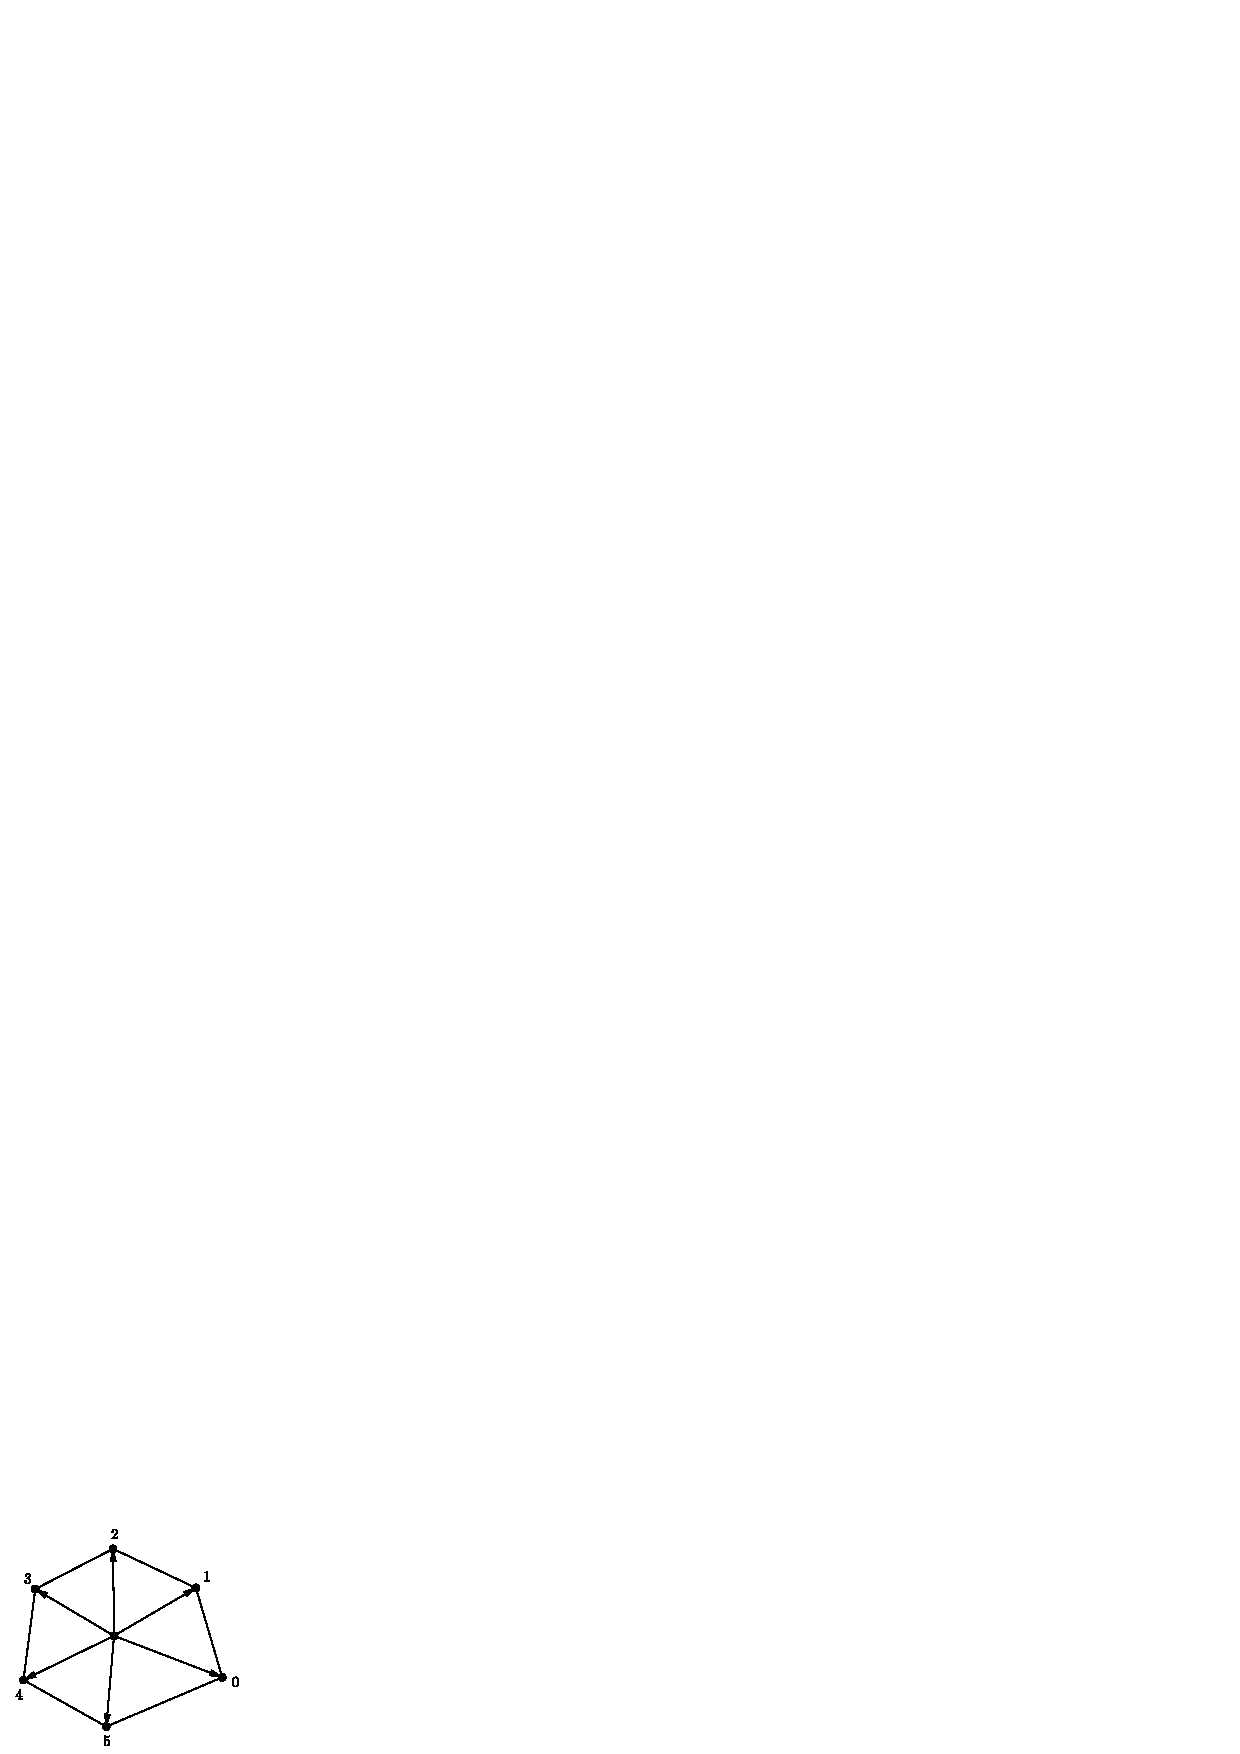
\includegraphics[width=0.5\linewidth]{struct.png}}
	\caption{Структура данных {\itshape <<Узлы с соседями>>}}
	\label{pic:struct}
\end{figure}

В нашей задаче будут часто производиться коррекции пучков сайтов,
поэтому операцию добавления и удаления ребер из пучка нужно производить очень эффективно.
В связи с этим требованием была выбрана структура данных {\itshape <<Узлы с соседями>>} (рис.\ref{pic:struct}).
Такая структура для каждого сайта хранит его координаты на плоскости и список номеров смежных сайтов в обходе против часовой стрелки.
Рассматриваемая структура данных неявно содержит ребра триангуляции, грани в данной структуре не хранятся вообще,
что в нашей задаче, вообще говоря, и не нужно.

\subsection{Построение разрезов и швов триангуляций Делоне}
Процесс построения разрезов и швов основан на проверке условия Делоне для ребер триангуляции,
которую можно осуществлять при помощи углового критерия (лемма \ref{th:lem1}) :

\begin{lemma}
\label{th:lem1}
Пусть $\textbf{S}$ --- множество сайтов, для пары $A, B \in \textbf{S}$ выполнено условие Делоне, тогда
для любых других двух сайтов $C, D \in \textbf{S}$, лежащих по разные стороны от $AB$, справедливо:
$\angle ACB + \angle ADB \le 180^\circ$ и $\angle ABD \ge \angle ACD$
\end{lemma}

\begin{proof}
Докажем, что если $AB$ --- ребро Делоне, то для любых других двух сайтов $C, D \in \textbf{S}$, лежащих по разные стороны от $AB$, справедливо
$\angle ACB + \angle ADB \le 180^\circ$ (рис. \ref{pic:l11}).

\begin{figure}[htb!]
	\center{\includegraphics[width=0.3\linewidth]{l11.png}}
	\caption{$\angle ACB + \angle ADB \le 180^\circ$}
	\label{pic:l11}
\end{figure}

Рассмотрим окружность, инцидентную сайтам $A$ и $B$, точка $E$ --- середина отрезка $AB$.
Отрезки $EC$ и $ED$ пересекают окружность в точках $C'$ и $D'$ соответственно.
Для четырехугольника $AC'BD'$ имеем $\angle AC'B + \angle AD'B = 180^\circ$, так как он вписан в окружность.
Если окружность пустая, то $\angle ACB \le \angle AC'B$ и $\angle ADB \le \angle AD'B$, откуда и получаем доказываемое утверждение:
$\angle ACB + \angle ADB \le \angle AC'B + \angle AD'B = 180^\circ$
если $\angle ACB + \angle ADB \ge 180^\circ$, то пустой окружности, инцидентной $A$ и $B$, не существует, что и доказывает утверждение.

Рассмотрим второе утверждение (рис. \ref{pic:l12}).

\begin{figure}[htb!]
	\center{\includegraphics[width=0.3\linewidth]{l12.png}}
	\caption{$\angle ABD \ge \angle ACD$}
	\label{pic:l12}
\end{figure}

Предположим противное, пусть $\angle ABD < \angle ACD$.
Построим описанную окружность для треугольника $ABD$, точка $С$ лежит внутри нее.
Пусть $C'$ --- точка пересечения прямой $CD$ с окружностью. В четырехугольнике $AC'BD$, вписанном в окружность,
имеем $\angle AC'B + \angle ADB = 180^\circ$.
Поскольку $\angle AC'B < \angle ACB$, получаем: $\angle ACB + \angle ADB > 180^\circ$.
А тогда для $AB$ согласно первому утверждению леммы не выполняется условие Делоне.
Значит, предположение неверно, то есть $\angle ABD \ge \angle ACD$.
\end{proof}

Пусть найдена разноцветная пара сайтов $A$ и $B$, такая что ребро $AB$ образует ребро Делоне в объединенной триангуляции,
ещё не включенное в нее.
Например, $AB$ является стартером.
Присоединение ребра $AB$ к пучкам сайтов-вершин $A$ и $B$ может привести к нарушению условия Делоне для некоторых ребер из этих пучков.
Все ребра, не удовлетворяющие условию Делоне должны быть разрушены на этом этапе.

Пусть $A$ --- левый, а $B$ --- правый сайты ребра Делоне $AB$.
Рассмотрим, как вставляется ребро $AB$ в пучок сайта A.

\begin{figure}[htb!]
	\center{\includegraphics[width=0.4\linewidth]{deleteWrongEdges.png}}
	\caption{Коррекция одноцветных ребер}
	\label{pic:deleteWrongEdges}
\end{figure}

Пусть $AC_1$ и $AC_2$ одноцветные ребра пучка A,
что сайты $B$, $C_1$ и $C_2$ идут в порядке обхода против часовой стрелки в пучке сайта $A$ (рис. \ref{pic:deleteWrongEdges}).
Для ребра $AC_1$ нарушено условие Делоне, если $\angle AC_2C_1 + \angle ABC_1 > 180^\circ$.
В этом случае ребро $AC_1$, а ребро $AC_2$ подвергается аналогичной проверке.
Если же для ребра $AC_1$ условие Делоне выполнено, то ребро $AC_1$ сохраняется в объединенной триангуляции и ребро $AC_2$ не тестируется.

Аналогичным образом выполняется коррекцию пучка сайта B, за исключением того,
что ребра рассматриваются в направлении по часовой стрелке.

Пучки, для которых выполнена описанная коррекция, будем называть {\itshape правильными}.
Рассмотрим процесс образования новых разноцветных ребер объединенной триангуляции Делоне:

\begin{lemma}
\label{th:lem2}
Пусть пучки сайтов $A$ и $B$ разноцветного ребра $AB$ являются правильными.
Точка $C$ следует за точкой в $B$ в пучке сайта $A$, точка $D$ предшествует точке $A$ в пучке сайта $B$,
тогда если $\angle ACB > \angle ADB$, то $CB$ является новым ребром Делоне, иначе $AD$ является новым ребром Делоне.
\end{lemma}

\begin{proof}
Для ребра $AB$ выполнено условие Делоне, значит, для него существует пустая окружность инцидентная сайтам $A$ и $B$ (рис. \ref{pic:l21}).
Рассмотрим описанные окружности треугольников $\triangle ACB$ и $\triangle ADB$.
Очевидно, что дуги этих окружностей, лежащие ниже $AB$, целиком попадают внутрь пустой окружности ребра $AB$,
значит, там не может оказаться ни один сайт.
Выше ребра $AB$ существует только одна пустая окружность, описанная вокруг $\triangle ACB$ или $\triangle ADB$,
причем та, у которой угол треугольника, опирающийся на сторону $AB$ больше.
То есть, если $\angle ACB > \angle ADB$, то $CB$ является новым ребром Делоне, иначе $AD$ является новым ребром Делоне.
\end{proof}

\begin{figure}[htb!]
	\center{\includegraphics[width=0.3\linewidth]{l21.png}}
	\caption{Создание новых разноцветных ребер}
	\label{pic:l21}
\end{figure}

Лемма \ref{th:lem2} описывает процесс образования новых разноцветных стежков при построении шва.
Из начального стежка $AB$ получаем следующий стежок $AD$ или $CB$.
Данный процесс схож с алгоритмом слияния разделенных триангуляций Ли-Шехтера \cite{Lee}.
Различия разделенных и неразделенных триангуляций состоят в том, что новая грань может быть пересечена ребрами исходных триангуляций.
Такие пересекающиеся ребра должны быть удалены во время построения очередного стежка.

Пусть $AB$ --- текущее разноцветное ребро Делоне, не ограничивая общности будем считать,
что $AD$ --- новое разноцветное ребро (рис. \ref{pic:triCorrection}).

\begin{figure}[htb!]
	\center{\includegraphics[width=0.3\linewidth]{triCorrection.png}}
	\caption{Пресечение ребер исходных триангуляций с новой гранью $\triangle ABD$}
	\label{pic:triCorrection}
\end{figure}

По лемме \ref{th:lem2} $AD$ не может иметь пересечений со старыми одноцветными ребрами из пучков сайтов $A$, $B$ и $D$.
Про два оставшихся ребра $AB$ и $BD$ так утверждать нельзя.
Действительно, все ребра в пучке $A$, лежащие между $AB$ и $AD$, обязательно пересекают одноцветное ребро $BD$,
по алгоритму построения ребра $AD$ все эти ребра не войдут в объединенную триангуляцию и должны быть разрушены.

Рассмотрим теперь пучок сайта $D$, в который включено вновь образованное ребро Делоне $AD$.
В этом пучке также могут найтись одноцветные ребра, лежащие между $DA$ и $DB$, которые пересекают ребро Делоне $AB$ и должны быть разрушены.
Поиск и разрушение указанных ребер осуществляется на основе последовательного просмотра пучка $A$ от $AB$ до $AD$ против часовой стрелки и пучка $D$ от $DA$ до $DB$ по часовой стрелке.

\begin{lemma}
\label{th:lem3}
Если сайт инцидентен разрушенному одноцветному ребру, то в объединенной триангуляции он инцидентен разноцветному ребру.
\end{lemma}

\begin{proof}
Рассмотрим одноцветное разрушенное ребро $AB$, имеющее инцидентную пустую окружность $C_1$ в исходной триангуляции.
Поскольку ребро было разрушено, значит, соответствующая окружность перестала быть пустой,
то есть в нее попали сайты другого цвета.

\begin{figure}[htb!]
	\center{\includegraphics[width=0.4\linewidth]{l31.png}}
	\caption{Пояснение к лемме \ref{th:lem3}}
	\label{pic:l31}
\end{figure}

Тогда, внутри этой окружности найдется сайт $D$ другого цвета, имеющий общую с сайтом $B$ инцидентную пустую окружность $C_2$ (рис. \ref{pic:l31}). Эта окружность лежит внутри окружности $C_1$ и имеет с ней общую касательную в точке $B$, значит, пара разноцветных сайтов $BD$ образует ребро Делоне, которое войдет в объединенную триангуляцию.
\end{proof}

Таким образом, мы описали алгоритм построения разреза и шва при условии, что найден стартер.

\subsection{Поиск стартеров}
В задаче поиска первого и последующих стартеров используется различная информация о триангуляциях.
Первый стартер ищется на основе начальной информации о триангуляциях,
поиск последующих использует информацию о уже построенных швах и разрушенных при этом одноцветных ребер.
В процессе поиска стартеров используются минимальные остовные деревья исходных триангуляций.
Об этом будет подробнее рассказано ниже.

Рассмотрим условия существования стартеров (разноцветных ребер Делоне).

\begin{lemma}
\label{th:lem4}
Сайт имеет инцидентное разноцветное ребро Делоне $\Leftrightarrow$ существует инцидентная ему окружность, внутри которой нет сайтов одного с ним цвета, но есть сайты противоположного цвета на ней или внутри нее.
\end{lemma}

\begin{figure}[htb!]
	\center{\includegraphics[width=0.4\linewidth]{starterLemma.png}}
	\caption{Условие существования стартера}
	\label{pic:starterLemma}
\end{figure}

\begin{proof}
Достаточность. Пусть для некоторого сайта $A$ существует инцидентная ему окружность с центром $C$,
внутри которой нет ни одного сайта того же цвета, что и $A$,
но есть сайты противоположного цвета $D_1, D_2, \ldots, D_k, k \ge 1$ другого цвета внутри или на окружности (рис. \ref{pic:starterLemma}).
Рассмотрим множество окружностей, инцидентных парам сайтов $A$ и $D_i, i = 1, \ldots, k$,
имеющих в точке $A$ общую касательную с окружностью с центром в точке $C$.
Окружность, имеющая минимальный радиус, является пустой, и она инцидентна разноцветной паре сайтов.
Значит, эта пара сайтов образует ребро Делоне и может являться стартером.

Необходимость. Есть пара сайтов, образующая ребро Делоне с инцидентной пустой окружностью.
Эта окружность и будет удовлетворять условию леммы.
\end{proof}

Согласно лемме \ref{th:lem4}, если существует сайт $A$ и инцидентная ему окружность $O$, удовлетворяющая условию леммы,
то поиск стартера сводится к перебору сайтов $D_1, D_2, \ldots, D_k, k \ge 1$, отличного от $A$ цвета,
внутри этой окружности и выбору сайта $D_{min}$,
такого что инцидентная $A$ и $D_{min}$ окружность имеет с окружностью $O$ общую касательную в точке $A$ и
минимальный радиус из всех таких окружностей, инцидентных $A$ и $D_i$.
Тогда ребро $AD_{min}$ можно использовать в качестве стартера.

\subsubsection{Поиск первого стартера}
Будем говорить, что сайт $A$ {\itshape лежит левее} сайта $B$,
если $A$ предшествует $B$ при лексикографическом упорядочивании сайтов по возрастанию координат $(x, y)$.

\begin{figure}[htb!]
	\center{\includegraphics[width=0.6\linewidth]{starterExample.png}}
	\caption{Поиск первого стартера}
	\label{pic:starterExample}
\end{figure}

Пусть $\textbf{B}$ и $\textbf{W}$ множества сайтов исходных триангуляций.
Найдем сайты $B_{min}$ и $W_{min}$, являющиеся самыми левыми в соответствующем множестве точек $\textbf{B}$ и $\textbf{W}$.
Не ограничивая общности, будем считать, что $B_{min}$ лежит левее, чем $W_{min}$  (рис. \ref{pic:starterExample}).
Рассмотрим окружность $O$, инцидентную сайтам $B_{min}$ и $W_{min}$ с центром на луче, параллельном оси $Ox$,
выходящим из точки $W_{min}$ влево.
Окружность $O$ не содержит ни одного сайта из $\textbf{W}$, потому что лежит левее самого левого сайта этого множества $W_{min}$,
и содержит сайт $B_{min}$ на границе окружности.
Возможно, ещё часть сайтов из $\textbf{B}$ попадет внутрь этой окружности.
Тогда точка $W_{min}$ и окружность $O$ удовлетворяют условиям леммы \ref{th:lem4}.
То есть первый стартер найден.

Время поиска сайтов складывается из вычисления самых левых точек множеств $\textbf{B}$ и $\textbf{W}$ и
перебора точек из множества $\textbf{B}$ по алгоритму из леммы \ref{th:lem4},
то есть линейно по общему числу сайтов.

\subsubsection{Минимальные остовные деревья}
Задача поиска последующих стартеров основана на использовании минимальных остовных деревьев исходных триангуляций Делоне.
Теоретическая оценка трудоемкости задачи построения минимального остова составляет $О(N\log N)$.
В то же время известно, что на основе триангуляции Делоне МОД может быть построен за линейное время.
Построение МОД исходных триангуляций Делоне выполняется с помощью алгоритма Черитона-Тарьяна \cite[стр. 278-280]{Preparata},
линейного по числу вершин триангуляций.
Пример ЕМОД для триангуляции Делоне показан на рис. \ref{pic:mst}.

\begin{figure}[htb!]
	\center{\includegraphics[width=0.5\linewidth]{mst.png}}
	\caption{Евклидово минимальное остовное дерево триангуляции Делоне}
	\label{pic:mst}
\end{figure}

Построение минимальных остовных деревьев осуществляется в процессе предобработки,
предшествующем непосредственному слиянию исходных триангуляций.
Рассмотрим подробнее алгоритм Черитона-Тарьяна.
{\itshape Лесом} называется упорядоченное множество деревьев.
На каждом шаге построения МОД алгоритм обрабатывает лес, содержащий несколько деревьев,
которые в ходе данного алгоритма станут поддеревьями искомого остовного дерева.
Сначала каждое дерево леса состоит из одной вершины триангуляции без ребер,
размер леса равен числу точек в триангуляции.
Для выбора дерева $T$ (которое будет объединено с другим деревом леса) они указали однородное правило выбора, перед использованием которого в очередь помещаются все деревья, содержащие по одной вершине.
\begin{enumerate}
	\item Выбрать дерево из начала очереди.
	\item Если дерево $T''$ получено в результате объединения дерева $T$ с некоторым другим деревом $T'$,
		то удалить $T$ и $T'$ из очереди и добавить $T''$ в конец очереди.
\end{enumerate}

Каждому дереву $T$ из очереди поставим в соответствие целое число, называемое {\itshape этапом} и вычисляемое следующим образом:
$stage(T) = 0$, если $|T| = 1$, и $stage(T)~=~\min(stage(T'),~stage(T''))~+~1$,
если $T$ является объединением деревьев $T'$ и $T''$.
В любой момент работы алгоритма последовательность чисел $stage(T)$ является неубывающей от начала к концу очереди.
Будем говорить, что этап $j$ завершен, если из очереди удалено дерево $T$,
для которого $stage(T) = j$, и ни для одного другого дерева $T$ в очереди значение $stage(T)$ не равно $j$.
После завершения этапа $j$ очередь содержит не более $\frac{N}{2^{j + 1}}$ элементов,
а всего имеется не более $\lceil\log_2N\rceil$ этапов.

Далее выбрав из очереди первый элемент $T$ ($stage(T) = j$), среди ребер,
соединяющих вершины дерева $T$ с вершинами вне его, ищем ребро наименьшей длины.
При такой организации обработки на каждом этапе каждое ребро просматривается не более двух раз
(кроме ребер, уже вошедших в некоторое дерево $T$).

Метод, позволяющий получить Евклидово МОД из триангуляции Делоне за линейное время,
использует операцию <<очистки>>, предложенную Черитоном и Тарьяном.
Цель операции очистки состоит в том, чтобы сжать исходный граф $G$ (граф триангуляции Делоне),
преобразовав его в некоторый граф $G^*$, который в любой момент работы алгоритма содержит лишь необходимую информацию.
Это означает, что каждое дерево $T$, входящее в лес $F$, сжимается в единственную вершину графа $G$
(т. е. удаляются все неотобранные ребра, соединяющие вершины дерева $T$) и
удаляются все ребра, за исключением самого короткого из неотобранных, соединяющие деревья $T'$ и $T''$.
Очистка графа производится сразу же после завершения этапа.
Предположим, что с каждым деревом $T$ связан список неотобранных ребер, инцидентных вершинам дерева $T$.
Формальное описание процедуры построения евклидова минимального остовного дерева описано в алгоритме \ref{alg:mst}.

\begin{algorithm}[htb!]
\caption{Построение ЕМОД по триангуляции Делоне}\label{emst}
\begin{algorithmic}[1]
\Procedure{EMST}{}
	\State $F := \emptyset$
	\For{$i := 1$ to $N$}
		\State $stage(p_i) := 0$
		\State $F.insert(p_i)$
	\EndFor
	\State $j := 1$
	\While{$F \not= \emptyset$}
		\State $T' := F.get()$
		\If{$stage(T') == j$}
            \State Очистить граф
            \State $j := j + 1$
        \EndIf
        \State $(u, v)$ --- кратчайшее из неотобранных ребер, инцидентных $T'$ ($u \in T'$)
        \State $T'' := $ дерево в $F$, содержащее $v$
        \State $T := merge(T', T'')$
        \State Удалить $T''$ из $F$
        \State $stage(T) := \min(stage(T'),~stage(T'')) + 1$
        \State $F.insert(T)$
	\EndWhile
\EndProcedure
\end{algorithmic}
\label{alg:mst}
\end{algorithm}

Поиск последующих стартеров основан на том, что при построении разреза в триангуляции Делоне нарушается ее связность,
при этом среди разрушенных ребер обязательно окажется ребро МОД этой триангуляции Делоне.

Будем называть окружность, диаметром которой является ребро МОД, {\itshape окружностью влияния ребра}.
Далее рассмотрим несколько свойств минимальных остовных деревьев.

\begin{lemma}
\label{th:lem5}
Окружность влияния ребра МОД является пустой окружностью ТД.
\end{lemma}

\begin{proof}
Предположим противное, пусть $AB$ --- ребро МОД, точка $C$ лежит внутри окружности с диаметром $AB$.
В $\triangle ABC~\angle C$ является тупым, поэтому $AC < AB$ и $BC < AB$.
Тогда если исключить ребро $AB$ из МОД, то дерево распадется на две связные компоненты,
в одной из которых будет находиться вершина $C$.
Если $С$ оказалась в одной компоненте с $A$, то включаем в дерево ребро $CB$ ($CB < AB$),
если $C$ находится в одной компоненте с $B$, меняем ребро $AB$ на $AC$.
После такого преобразования получаем дерево, суммарная длина всех ребер которого меньше, чем у исходного дерева,
что противоречит принадлежности ребра $AB$ к МОД, то есть утверждение доказано.
\end{proof}

\begin{lemma}
\label{th:lem6}
Расстояние между центрами двух ребер МОД не меньше, чем половина длины каждого ребра.
\end{lemma}

\begin{proof}
Предположим противное.
Пусть $AA_1$ и $BB_1$ --- ребра МОД с серединами $A_0$ и $B_0$, таки что $A_0B_0 \le AA_0$ (рис. \ref{pic:lem6}),
тогда их окружности влияния пересекаются в некоторых точках $C$ и $D$.
Предположим, что $AB \ge A_1B_1$.
Из точки $C$ проведем диаметры $CE$ и $CF$ кругов $A_0$ и $B_0$ соответственно.
В $\triangle CDE$ угол $\angle CDE$ прямой, а в $\triangle CDF$ угол $\angle CDF$ тоже прямой,
значит, $EF$ проходит через точку $D$.

\begin{figure}[htb!]
	\center{\includegraphics[width=0.4\linewidth]{lem6.png}}
	\caption{Пояснение к лемме \ref{th:lem6}}
	\label{pic:lem6}
\end{figure}

Из леммы \ref{th:lem5} следует, что точка $A$ лежит на дуге $ED$, а точка $B$ --- на дуге $DF$.
Углы $\angle EAD$ и $\angle DBF$ тупые, поскольку дуги $ED$ и $DF$ меньше полуокружностей.
Следовательно, $AB < AD + DB < ED + DF = EF = 2A_0B_0$, т.е. $AB < AA_1$.
Поскольку $A_1B_1 \le AB$, то и $A_1B_1 < AA_1$.

Покажем, что в этом случае $AA_1$ не может быть ребром МОД.
Действительно, если удалить из покрывающего дерева ребро $AA_1$,
то одна из точек $A$ или $A_1$ окажется в одной компоненте с ребром $BB_1$.
Если это точка $A$, то заменяем $AA_1$ на $A_1B_1$,
если это точка $A_1$, то заменяем $AA_1$ на $AB$.
В обоих случаях суммарная длина МОД уменьшается.
Полученное противоречие доказывает утверждение леммы. 
\end{proof}

\subsubsection{Поиск последующих стартеров}
{\itshape Мостами} будем называть ребра исходных триангуляций,
входящие в МОД, разрушенные при построении очередного разреза.
Сайт, инцидентный мосту, называется {\itshape свободным}, если он имеет только одноцветные инцидентные ребра.
Сайт называется {\itshape закрепленным}, если он инцидентен мосту, но среди инцидентных ему ребер есть разноцветные.
Свободные сайты могут быть присоединены к объединенной триангуляции только при помощи построения новых швов,
поэтому существование свободного сайта говорит о том,
что построение объединенной триангуляции ещё не завершено.

\begin{lemma}
\label{th:lem7}
Существует стартер, инцидентный свободному сайту.
\end{lemma}

\begin{proof}
Рассмотрим мост, инцидентный свободному сайту.
По определению он является ребром МОД одной из исходных триангуляций, тогда, согласно лемме \ref{th:lem5},
внутри окружности влияния моста нет сайтов одного с ним цвета.
Поскольку это ребро было разрушено при построении разреза, это означает,
что внутрь этой окружности попали сайты противоположного цвета.
Значит, для свободного сайта выполнены условия леммы \ref{th:lem4},
которая гарантирует существование стартера.
\end{proof}

Пусть сайты $A$ и $B$ --- разноцветные, сайт $A$ входит в триангуляцию Делоне $T$.
{\itshape Максимальными пустыми окружностями} будем называть пустые окружности,
которые не содержатся внутри других пустых окружностей, не совпадающих с ними.
Рассмотрим множество окружностей, инцидентных $A$ и являющихся пустыми относительно сайтов триангуляции $T$.
В этом множестве существую максимальные пустые окружности, которые являются описанными окружностями граней триангуляции $T$,
инцидентные сайту $A$. 
В случае, когда $A$ принадлежит границе выпуклой оболочки триангуляции Делоне $T$,
несобственные окружности также будут максимальными пустыми окружностями, инцидентными сайту $A$.

\begin{lemma}
\label{th:lem8}
Пусть $AB$ --- стартер. Тогда сайт $B$ попадает внутрь хотя бы одной из максимальных пустых окружностей в $T$, инцидентных сайту $A$.
\end{lemma}

\begin{proof}
Любая пустая окружность, инцидентная сайту $A$, принадлежит объединению максимальных пустых окружностей сайта $A$.
Если сайты $A$ и $B$ образуют ребро Делоне, то инцидентная им пустая окружность лежит также в этом объединении, откуда
и следует утверждение леммы.
\end{proof}

\begin{figure}[htb!]
	\center{\includegraphics[width=0.6\linewidth]{nextStarter.png}}
	\caption{Поиск последующих стартеров}
	\label{pic:nextStarter}
\end{figure}

Пусть $AB$ --- мост, сайт $A$ является закрепленным, сайт $B$ --- свободным (рис. \ref{pic:nextStarter}).
Сайты $A$ и $B$ имеют один и тот же цвет (на рисунке – черный) и в окружности влияния моста находятся лишь сайты противоположного цвета.
Согласно лемме \ref{th:lem7} свободный сайт $B$ может быть выбран в качестве первого сайта стартера.
Сайт $B$ попадает внутрь максимальных пустых окружностей триангуляции белых сайтов.
На рисунке это описанные окружности треугольных граней $\triangle C_3C_4C_5,~\triangle C_3C_5C_6,~\triangle C_6C_5C_7$.
Согласно лемме \ref{th:lem8} для нахождения второго сайта стартера можно выполнять перебор не по всем вершинам,
а только по вершинам граней, внутри описанных окружностей которых лежит сайт $B$.
Таким образом, поиск второго сайта осуществляется среди вершин этих граней,
причем только тех из них, которые попадают внутрь круга влияния моста,
в нашем примере среди сайтов $C_3, C_4$ и $C_6$.

Поскольку закрепленный сайт $A$ уже включен в объединенную триангуляцию,
а свободный сайт $B$ не включен, можно оценить положение $B$ относительно этой триангуляции.
Сайт $B$ либо попадает внутрь какой-то грани, либо лежит вне выпуклой оболочки второй триангуляции.
В последнем случае можно найти ребро выпуклой оболочки, определяющее полуплоскость, в которой лежит $B$.
Задачу определения местоположения свободного сайта относительно триангуляции,
в которую уже включен закрепленный сайт, будем называть {\itshape локализацией моста}.
Рассмотрим множество ребер триангуляции, которые пересекает мост.
Эти ребра естественным образом упорядочиваются в направлении от закрепленного сайта к свободному.
Легко видеть, что последнее из пересекаемых мостом ребер либо инцидентно треугольной грани,
содержащей сайт $B$, либо определяет полуплоскость, содержащую $B$.
Найденная грань или полуплоскость есть решение задачи локализации моста.
Таким образом, задача локализации моста решается путем трассировки ребер и граней триангуляции вдоль моста.

Найденная грань имеет описанную окружность, которая содержит свободный сайт $B$.
Поиск остальных граней триангуляции, чьи описанные окружности содержат $B$,
осуществляется путем проверки смежных граней.
Объединением этих граней является многоугольник, содержащий сайт $B$.
В рассматриваемом примере это многоугольник $C_3C_4C_5C_7C_6$.
Среди вершин многоугольника обязательно найдутся сайты,
лежащие внутри окружности влияния моста (в противном случае мост не был бы разрушен).
Один из этих сайтов и образует стартер вместе с сайтом $B$.

Таким образом, поиск стартера на основе свободного сайта и инцидентного ему моста может быть осуществлен следующим алгоритмом:

\begin{enumerate}
	\item Направленным перебором вдоль моста ищем грань триангуляции, в окружность которой попадает свободный сайт
	\item Находим все смежные грани триангуляции, в описанные окружности которых попадает свободный сайт
	\item Среди вершин этих граней определяем те сайты, которые попадают в окружность влияния моста
	\item Из найденных сайтов выбираем тот, который соответствует окружности минимального радиуса с центром на линии моста,
		инцидентной этому сайту и свободному сайту
\end{enumerate}

\section{Оценка вычислительной сложности алгоритма}
Алгоритм слияния перекрывающихся триангуляций Делоне можно разделить на три части:
построение минимальных остовных триангуляций Делоне,
поиск стартеров, построение разрезов и швов.
Алгоритм построения МОД Черитона-Тарьяна имеет сложность $O(n)$, что было показано выше.
Вычислительную сложность других частей алгоритма рассмотрим более подробно.

\subsection{Сложность поиска стартеров}
Пусть $n = |\textbf{B}| + |\textbf{W}|$ --- общее количество сайтов объединенной триангуляции.
Поиск начального стартера реализуется с временем $O(n)$ в худшем случае.
Поиск последующих стартеров включает в себя два перебора точек:
во-первых, это выбор моста –-- ребра МОД, разрушенного при разрезании триангуляций,
во-вторых, это пересечение мостом ребер триангуляции при локализации моста.
Можно построить примеры таких <<худших случаев>>, когда число мостов окажется $O(n)$ и
число ребер объединенной триангуляции, пересекающих отдельный мост, также $O(n)$.
Ниже будет показано, что общее число всех пересечений мостов и ребер исходных триангуляций все равно имеет сложность $O(n)$.

Рассмотрим процесс выбора очередного моста для трассировки.
Число ребер МОД равно $O(n)$.
Разрушенные при построении шва ребра МОД заносятся в отдельный список.
Если при сшивке оба сайта ребра становятся закрепленными, то ребро больше не входит в этот список.
В качестве очередного моста для трассировки выбирается первое ребро из этого списка, что требует времени $O(1)$.

Пусть разрезана одна из исходных триангуляций, например, $Del(\textbf{W})$ и разрез разбил ее на две компоненты.
В таком случае хотя бы одно из ребер МОД окажется разрушенным.
Из лемм \ref{th:lem5} и \ref{th:lem6} следует,
что внутри окружности влияния моста не могут находиться концевые и серединные точки других мостов.
Это позволяет оценить меру пересечения одного моста с окружностью влияния другого моста.

\begin{lemma}
\label{th:lem9}
Мост может вырезать из окружности влияния другого моста дугу размером не более $60^\circ$.
\end{lemma}

\begin{proof}
Пусть $AA_1$ и $BB_1$ --- мосты с серединами $A_0$ и $B_0$ соответственно,
а $D_1$ и $D_2$ --- точки пересечения $AA_1$ и окружности влияния моста $BB_1$.
Из лемм \ref{th:lem5} и \ref{th:lem6} получаем, точки $A_0$, $A$ и $A_1$ лежат вне окружности $B_0$.
Следовательно, отрезок $D_1D_2$ целиком лежит на $AA_0$ или $A_0A_1$.
Пусть для определенности $D_1D_2$ лежит на отрезке $AA_0$, тогда $D_1D_2 \le AA_0$.
В треугольнике $\triangle AA_0B_0$ сторона $AA_0$ не превосходит по длине стороны $AB_0$ и $A_0B_0$.
Следовательно, $\angle AB_0A_0 \le 60^\circ$.
Но тогда и $D_1B_0D_2 \le 60^\circ$, что и доказывает утверждение леммы. 
\end{proof}

\begin{figure}[htb!]
	\begin{minipage}[h]{0.32\linewidth}
		\center{\includegraphics[width=1.1\linewidth]{lem9.png}}
		\caption{Лемма \ref{th:lem9}}
		\label{pic:lem9}
	\end{minipage}
	\hfill
	\begin{minipage}[h]{0.32\linewidth}
		\center{\includegraphics[width=1\linewidth]{lem10.png}}
		\caption{Лемма \ref{th:lem10}}
		\label{pic:lem10}
	\end{minipage}
	\begin{minipage}[h]{0.32\linewidth}
		\center{\includegraphics[width=0.9\linewidth]{lem11.png}}
		\caption{Лемма \ref{th:lem11}}
		\label{pic:lem11}
	\end{minipage}
\end{figure}

Приведем следующие леммы без доказательства.

\begin{lemma}
\label{th:lem10}
Если два моста $AA_1$ и $BB_1$ одной ТД пересекают ребро $PQ$ другой ТД (рис. \ref{pic:lem10})
и концевая точка $P$ ребра попадает внутрь обеих окружностей влияния мостов,
то разность углов $APA_1$ и $BPB_1$ не меньше $60^\circ$.
\end{lemma}

\begin{lemma}
\label{th:lem11}
Если ребро ТД пересекает несколько мостов другой ТД, то концевая
точка ребра может попасть внутрь окружностей влияния не более чем двух мостов.
\end{lemma}

\begin{theorem}
\label{th:th1}
При объединении двух ТД каждое ребро пересекается не более чем с четырьмя мостами, которые оно разрушает.
\end{theorem}

\begin{proof}
Утверждение теоремы непосредственно следует из леммы \ref{th:lem11}.
Поскольку разрушение моста ребром происходит лишь при попадании конца ребра внутрь окружности влияния моста,
а по лемме один конец ребра может попасть лишь в две такие окружности,
общее число разрушенных одним ребром мостов не превышает четыре.
\end{proof}

Теорема \ref{th:th1} позволяет оценить общее время поиска всех стартеров.
При локализации моста осуществляется анализ всех пересечений моста с ребрами объединенной триангуляции.
При этом сам мост является одноцветным ребром одной из исходных триангуляций,
а пересекаемые им ребра являются либо разноцветными,
либо одноцветными, но противоположного цвета с мостом.
Если два отрезка пересекаются и каждый из них является ребром Делоне в своей триангуляции,
то в объединенную триангуляцию один из них не должен входить.
Это прямо следует из леммы \ref{th:lem1}.
Следовательно, либо мост разрушает ребро, либо ребро разрушает мост.
Те ребра, которые мост разрушает, имеют одно пересечение с одним мостом,
так как к моменту анализа следующего моста эти ребра уже разрушены.
Те ребра, которые сами разрушают мост, могут разрушить не более четырех мостов каждое.
Следовательно, общее количество пересечений мостов с ребрами не может превысить пятикратное число ребер во всех триангуляциях,
т.е. составляет O(n).
Таким образом, справедлива следующая теорема.

\begin{theorem}
\label{th:th2}
Вычислительная сложность алгоритма поиска всех стартеров составляет $O(n)$.
\end{theorem}

\begin{proof}
Доказательство этой теоремы прямо следует из вышеизложенных рассуждений.
\end{proof}

\subsection{Сложность построения разрезов и швов}
На этом шаге алгоритма разрушаются одноцветные ребра,
которые перестали удовлетворять условию Делоне в объединенной триангуляции,
и строятся разноцветные ребра.
Построение нового ребра осуществляется на основе углового критерия (лемма \ref{th:lem1}) для пары конкурирующих ребер,
т.е. занимает фиксированное время $O(1)$.
Для каждого нового разноцветного ребра выполняется оценка корректности соседних с ним одноцветных ребер.
Такая проверка дважды запускает угловой критерий.
Если по результатам тестирования какое-то ребро уничтожается, то ставшее соседним другое одноцветное ребро вновь подвергается тесту.
Таким образом, время на уничтожение одного одноцветного ребра также оценивается как постоянное $O(1)$.

В баланс времени следует включить еще время выполнения операций по включению новых ребер в пучки их концевых сайтов.
При включении первого стежка, образуемого из стартера, может потребоваться полный перебор всех ребер, входящих в пучки двух инцидентных ему сайтов. Поэтому, общее время включения всех начальных ребер в пучки оценивается как $O(n)$.
А вот включение каждого очередного ребра уже не требует перебора ребер,
поскольку новое ребро устанавливается в пучок вслед за текущим анализируемым ребром.
Поэтому общее время на включение всех ребер есть $O(n)$.

Общее число построенных ребер не превосходит количество ребер в выходной триангуляции,то есть $O(n)$,
а общее число разрушенных ребер не превосходит общее число ребер в исходных триангуляциях --- тоже $O(n)$.

Таким образом, с учетом теоремы \ref{th:th2} доказана следующая теорема.

\begin{theorem}
Предложенный алгоритм объединяет две неразделенные триангуляции Делоне за время O(n).
\end{theorem}

\section{Эксперименты}
В данном разделе будет описана программная реализация рассматриваемого алгоритма.
Проведен ряд экспериментов по замеру времени работы алгоритма на входных данных разного размера.

\subsection{Программная реализация}
Алгоритм слияния перекрывающихся триангуляций Делоне был реализован на языке программирования Python.

Структура данных, как наиболее важная часть реализации, хранится в следующем виде:
для каждого сайта исходных триангуляций имеется циклический список инцидентных сайтов,
упорядоченных в порядке обхода против часовой стрелки.

Для решения поставленной задачи был разработан макет программы,
позволяющий по входному множеству точек строить триангуляцию Делоне и минимальное остовное дерево,
а также слияние двух триангуляций Делоне.
Исходные множества точек могут быть введены вручную или сгенерированы автоматически.

\subsection{Вычислительный эксперимент}
Для проверки корректности работы алгоритма были проведены вычислительные эксперименты.
Случайным образом были сгенерированы два множества точек разного размера.
Тестирование на множествах точек, для которых $n < 1000$ почти бесполезно,
алгоритм работает очень быстро.
Эксперимент проводился на множествах точек, для которых $n \ge 10000$,
то есть каждое исходное множество триангуляций содержало не менее 5000 точек.

График замера времени показан на рисунке \ref{pic:timeWork}.
Видно, что график похож на линейный, что доказывает линейность работы алгоритма.

\begin{figure}[htb!]
	\center{\includegraphics[width=0.5\linewidth]{timeWork.png}}
	\caption{Время работы алгоритма слияния триангуляций}
	\label{pic:timeWork}
\end{figure}

\section{Заключение}
В данной работе был рассмотрен алгоритм слияния перекрывающихся триангуляций Делоне.
Вычислительный эксперимент подтверждает корректность работы алгоритма.
На защиту выносятся:

\begin{enumerate}
	\item Подробное описание алгоритма
	\item Разработка структур данных
	\item Разработка алгоритма слияния перекрывающихся триангуляций Делоне за линейное время
	\item Программная реализация слияния на простых примерах
\end{enumerate}

\newpage

\addcontentsline{toc}{section}{Использованная литература}

\bibliographystyle{utf8gost705u}
\bibliography{report_diploma}
\end{document}